\section{Frequency mode 13}
\label{FM13}
\subsection{Spectra}
\label{FM13:spectra}
Yearly median spectra for summer and winter are shown in
Fig.~\ref{fig:spectra:13}. Close-ups of the water-vapour peak around
$556.936\,\mathrm{GHz}$ (Fig.~\ref{fig:spectra:13:closeup}) show that the peak
appears to vary both in height and width. It can also be seen that the peak
appears to be shifted $1.5\,\mathrm{GHz}$ to the right compared to what would
be expected from simulations. This holds borth for spectra from FM~13 and
FM~113. The same is seen for the small \chem{O_3} peak.\todo{check O3 against
sims again} It is noted here that the spectra from FM~19 and FM~119 don't
exhibit this shift.


\begin{figure}[h]
    \centering
    \begin{subfigure}[b]{0.9545\textwidth}
        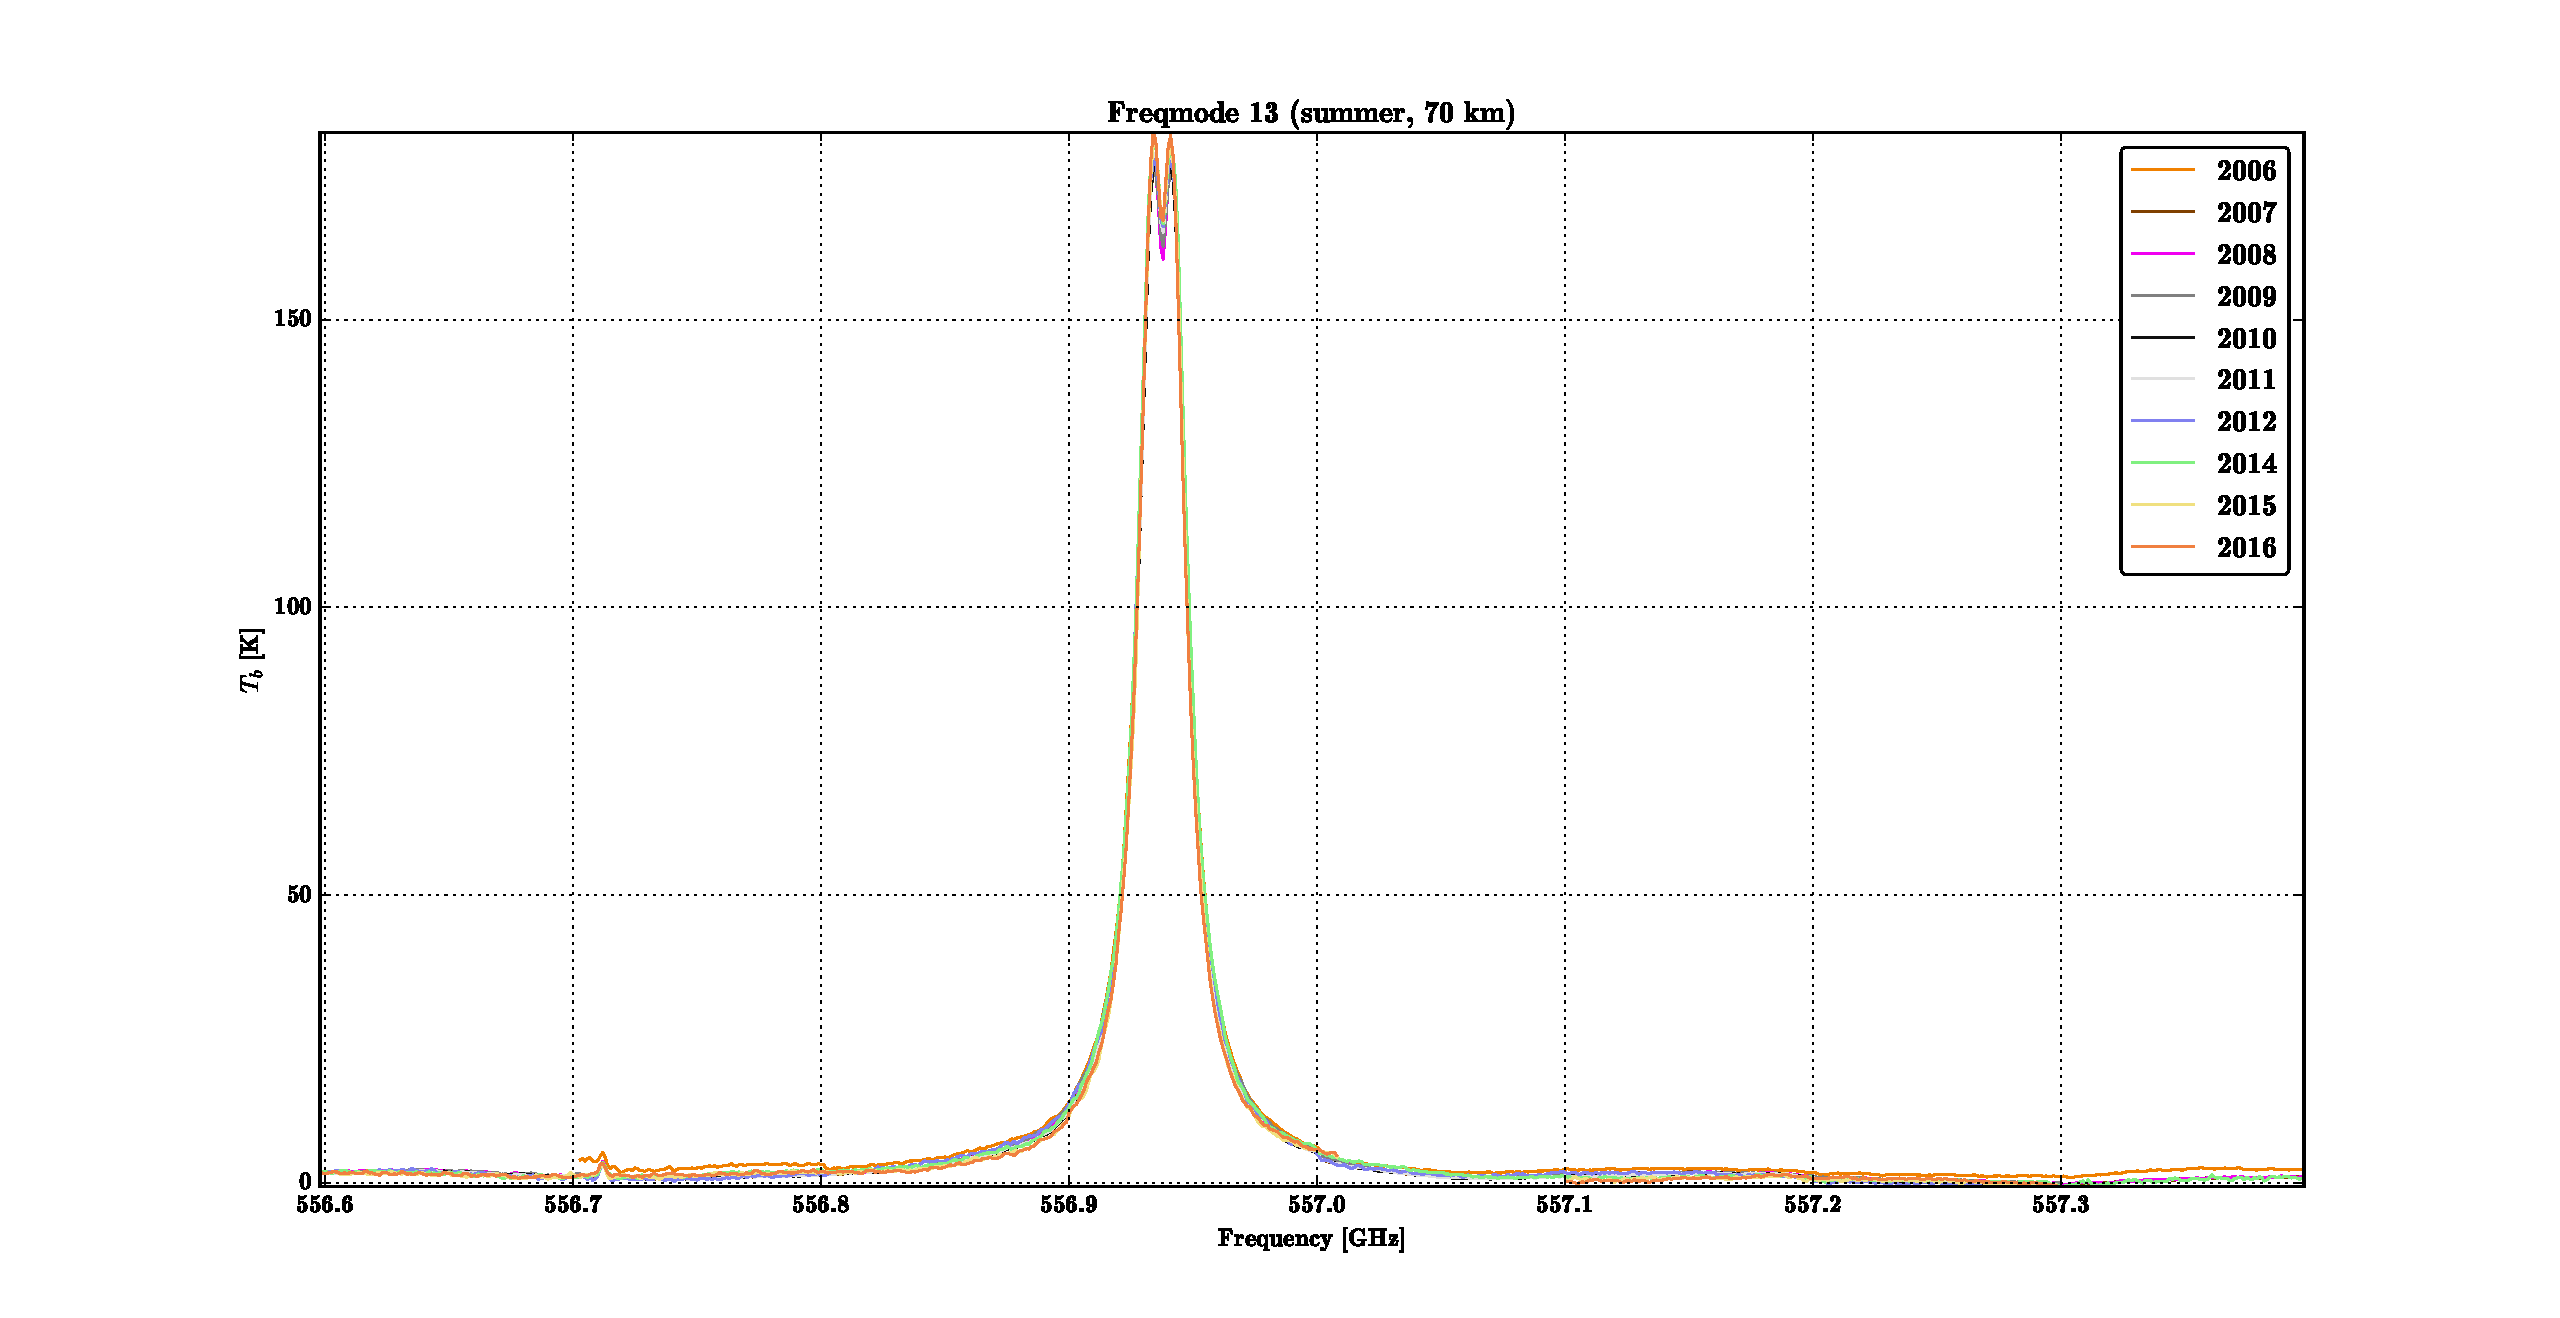
\includegraphics[width=\textwidth]{fm_13_spectra_summer.pdf}
        \caption{summer; 2014--2016 from FM~113}\label{fig:spectra:13:summer}
    \end{subfigure}
    \begin{subfigure}[b]{0.9545\textwidth}
        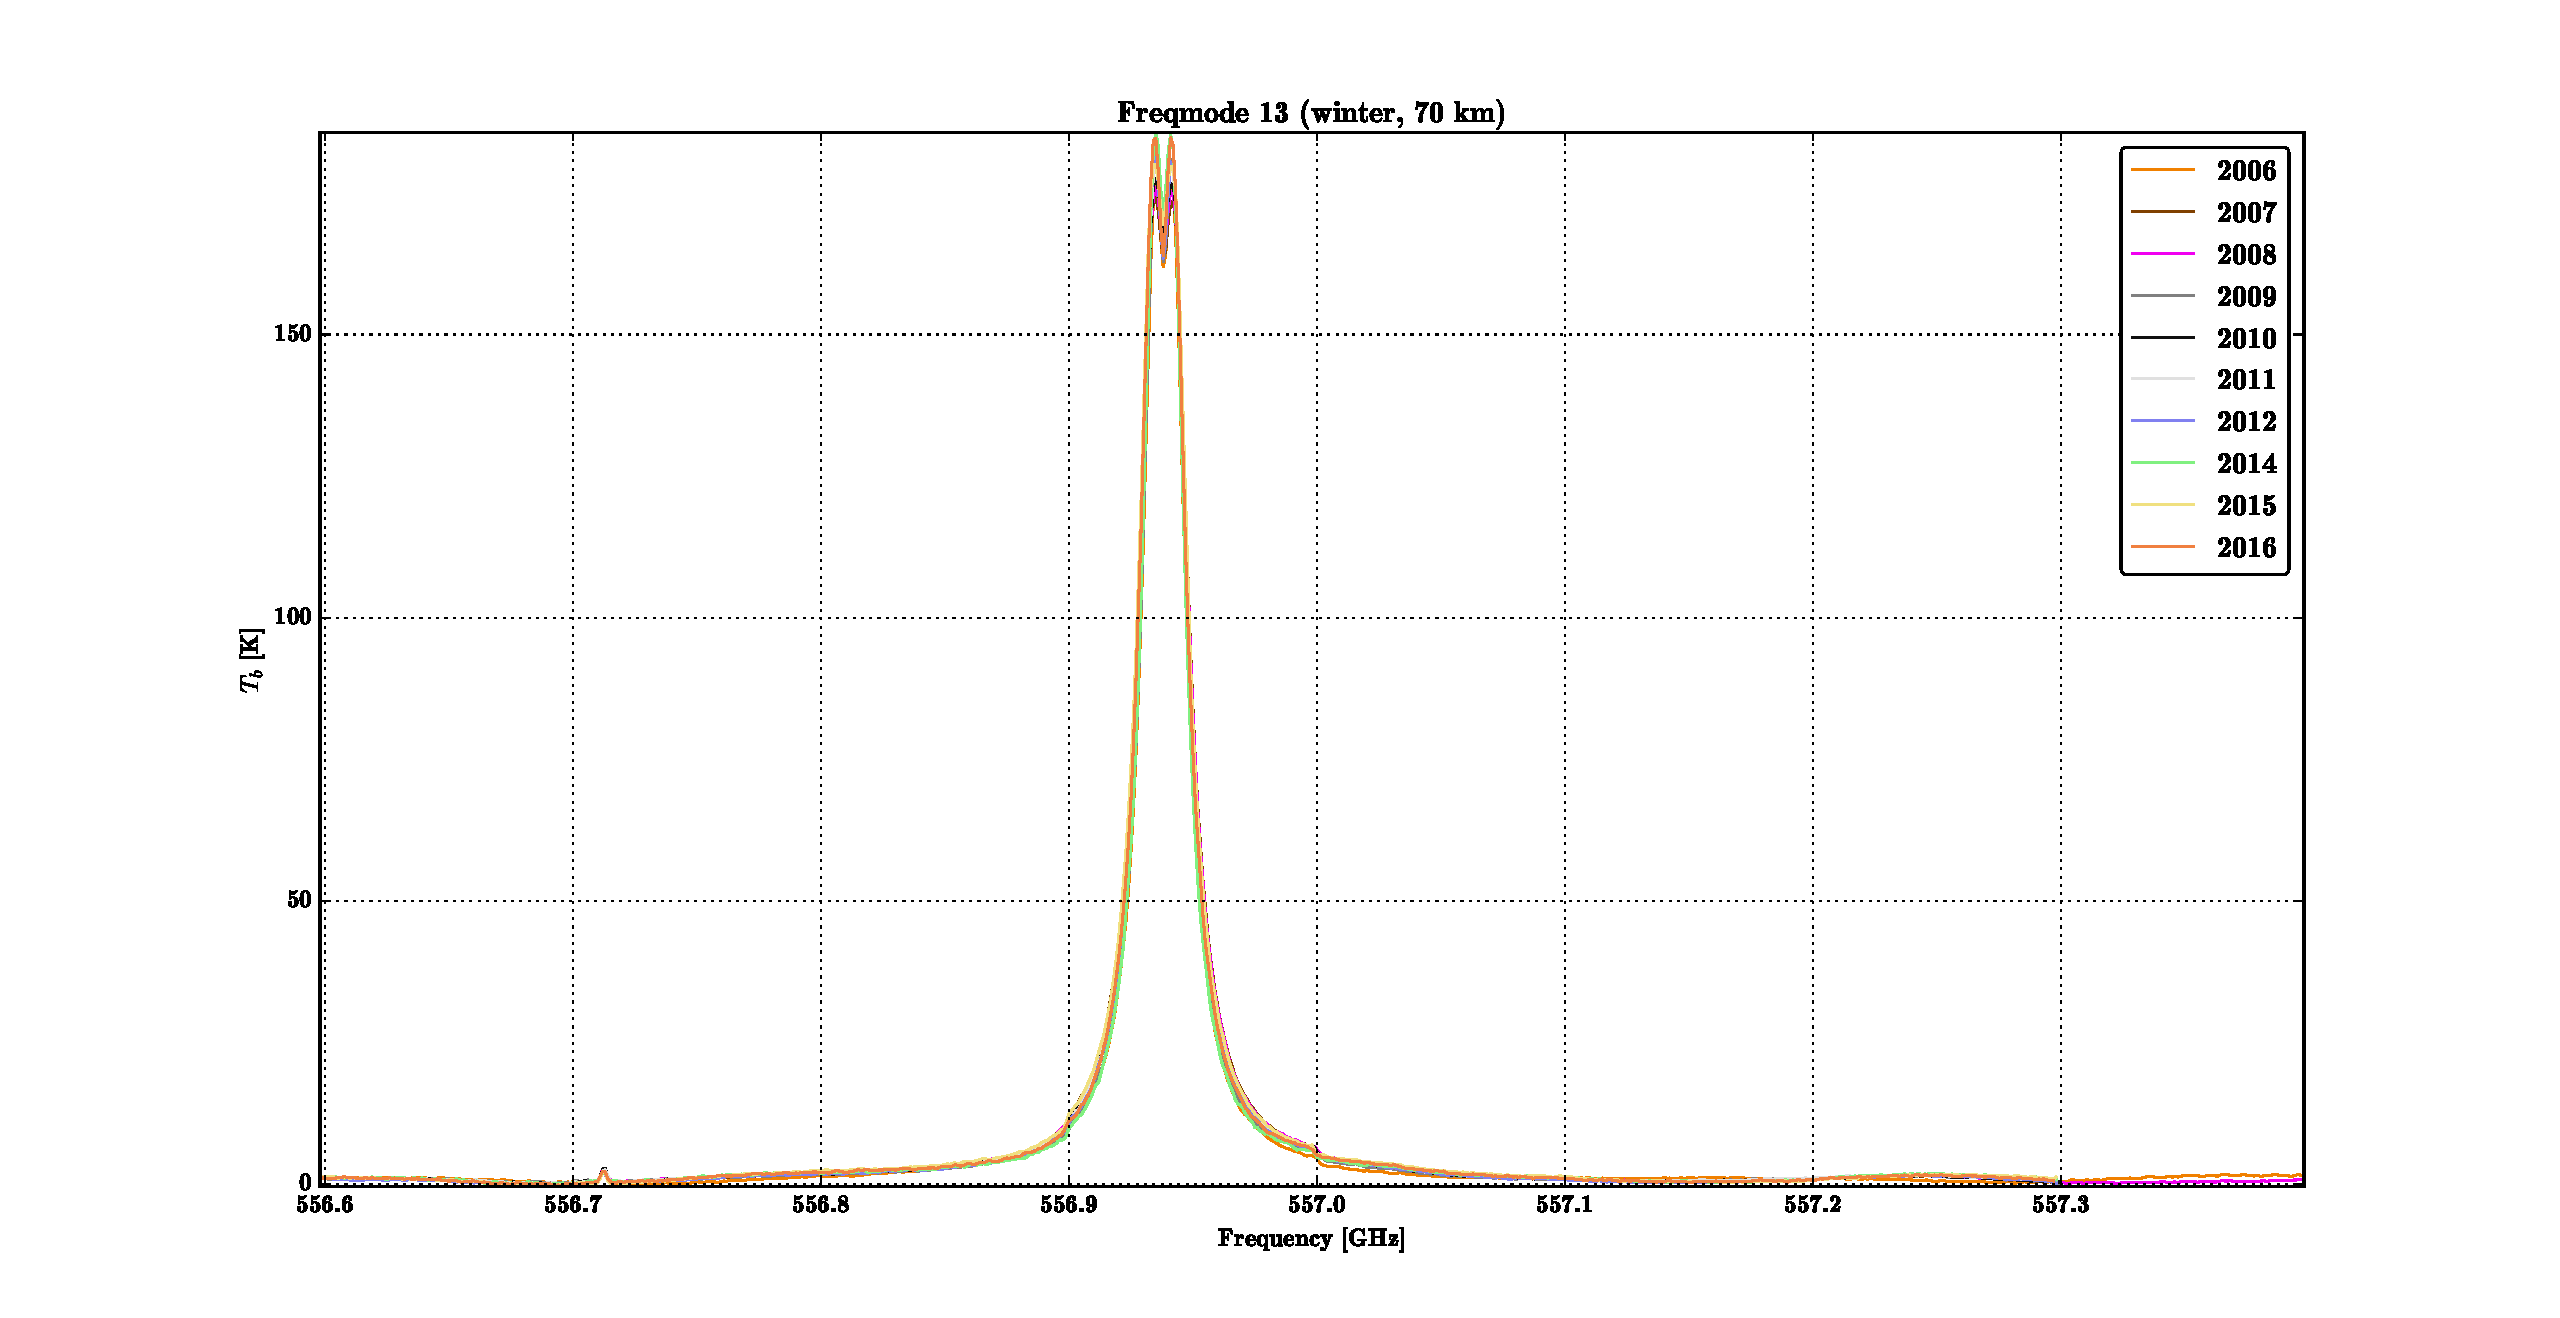
\includegraphics[width=\textwidth]{fm_13_spectra_winter.pdf}
        \caption{winter}\label{fig:spectra:13:winter}
    \end{subfigure}
    \caption{Annual median spectra for frequency~mode~13 for altitude
        interval 65--75~km. The large ``double peak'' in the middle is
        \chem{H_2O}, the small peak on the left is \chem{O_3}. The
        unhealthy sub-bands 1 and 2 are off to the very right, starting at
        $\sim557.2\,\mathrm{GHz}$.}\label{fig:spectra:13}
\end{figure}

\begin{figure}[h]
    \centering
    \begin{subfigure}[b]{0.9545\textwidth}
        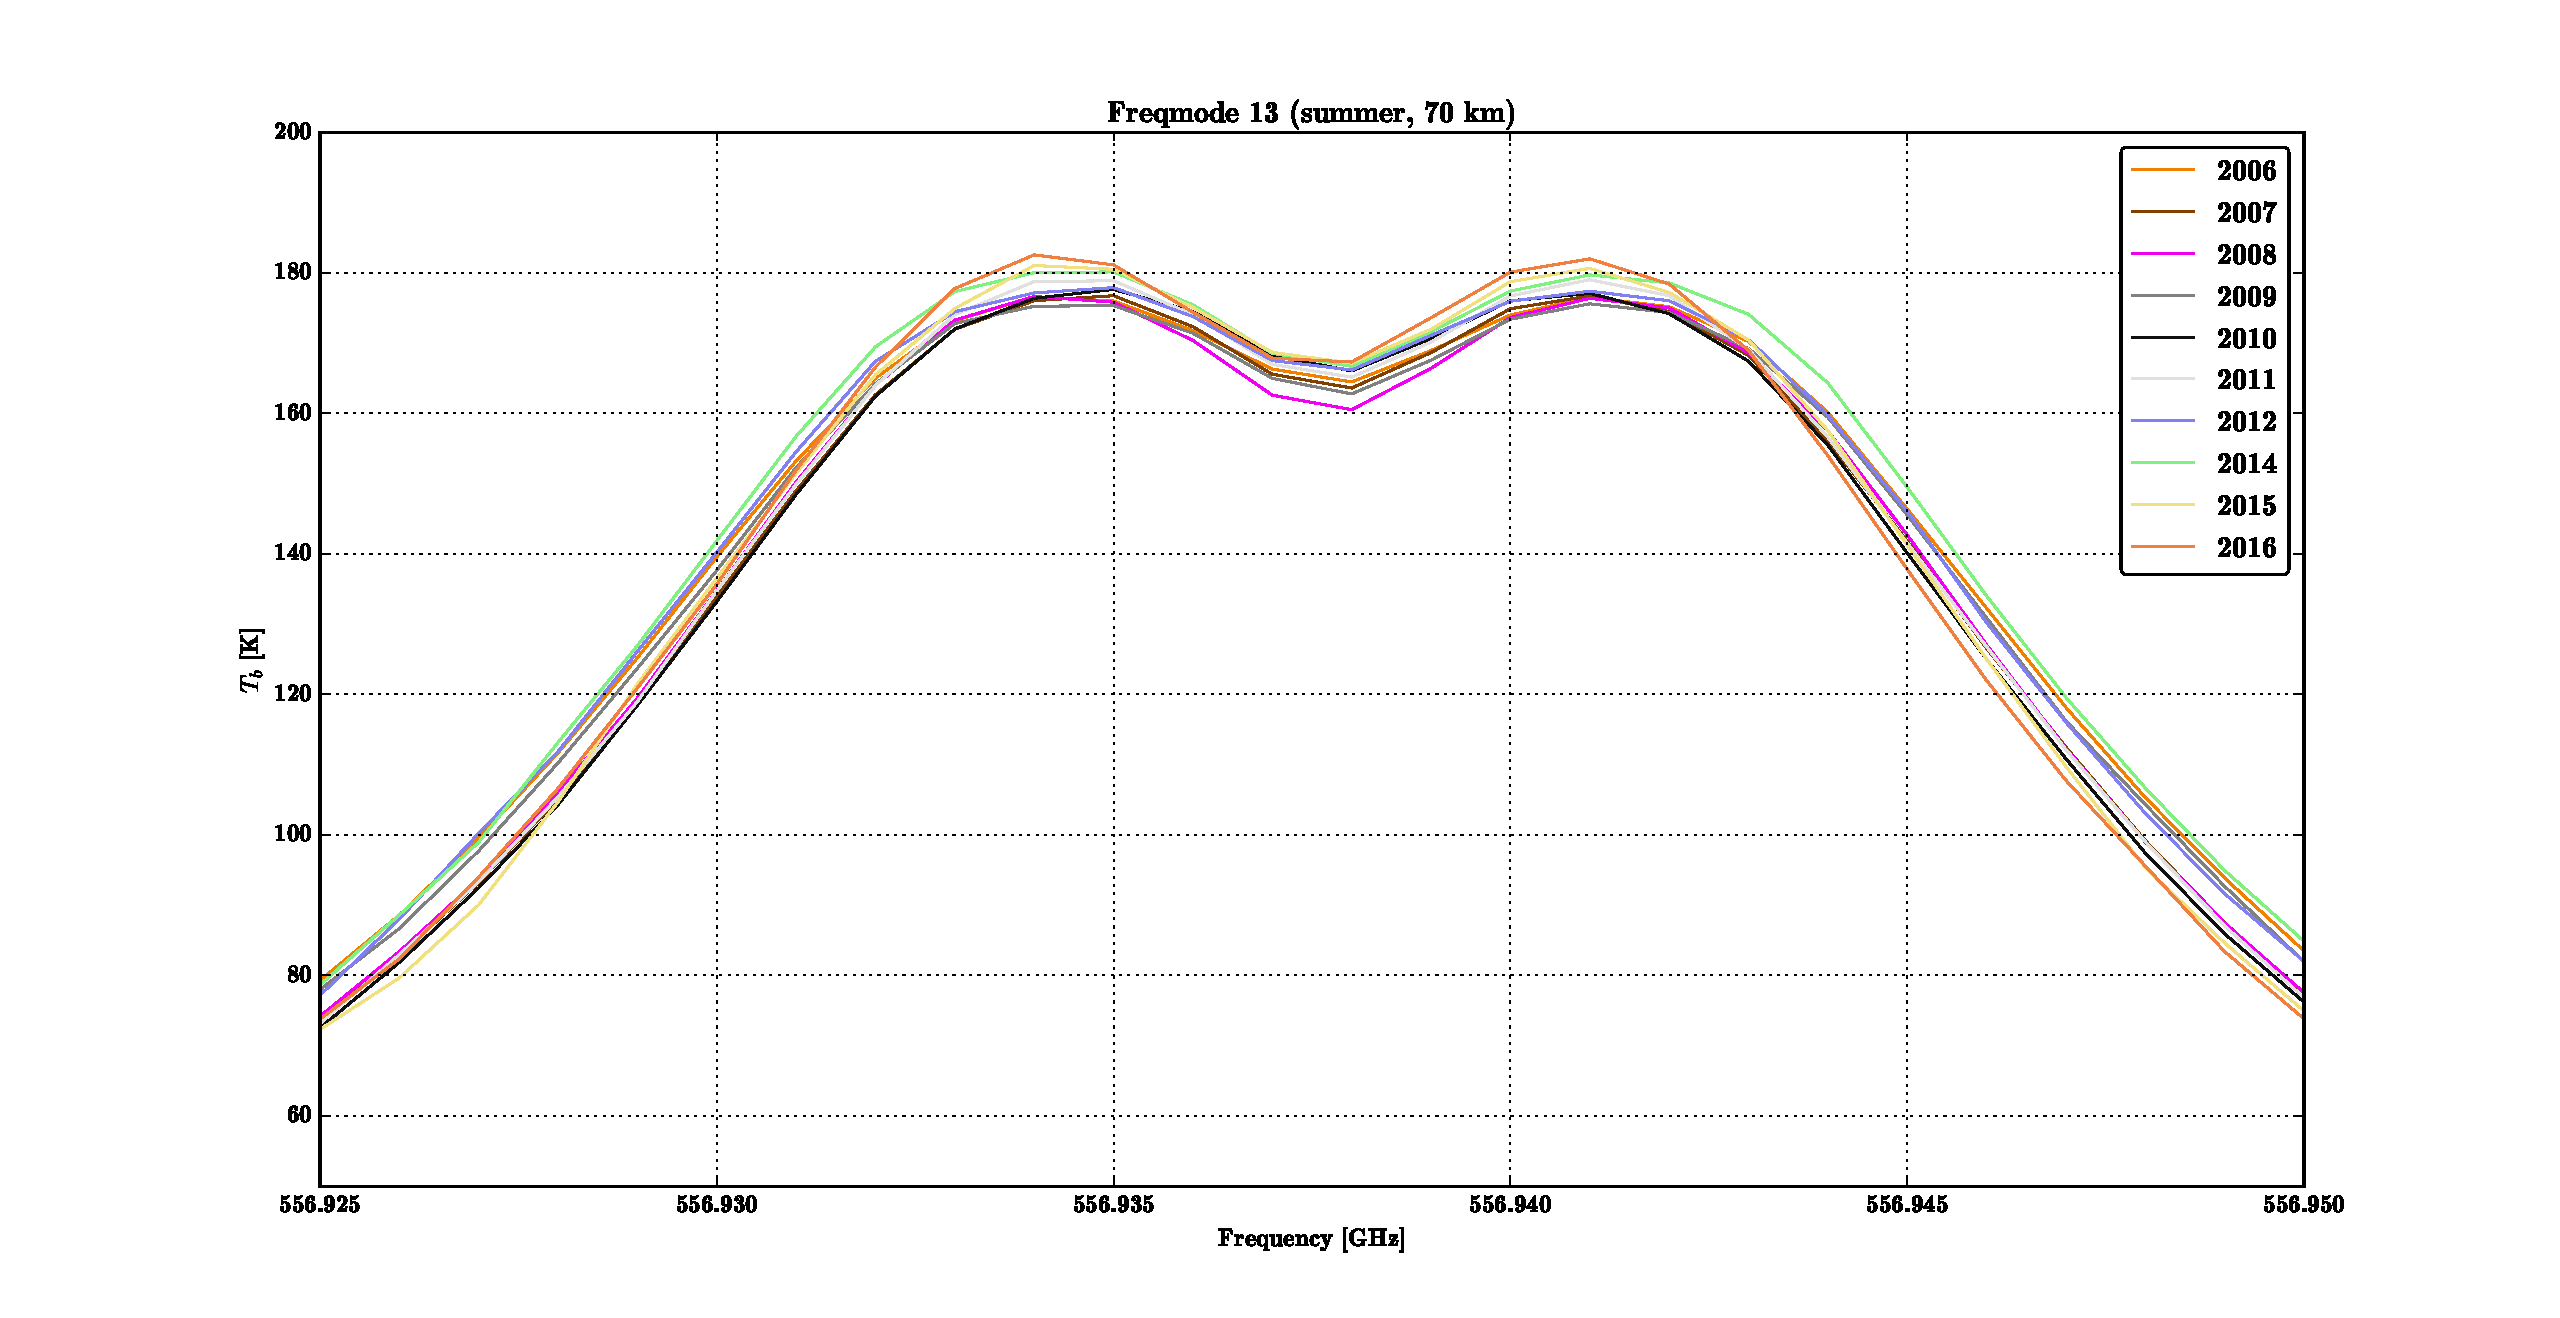
\includegraphics[width=\textwidth]{fm_13_spectra_summer_zoom.pdf}
        \caption{summer; 2014--2016 from
            FM~113}\label{fig:spectra:13:summer:closeup}
    \end{subfigure}
    \begin{subfigure}[b]{0.9545\textwidth}
        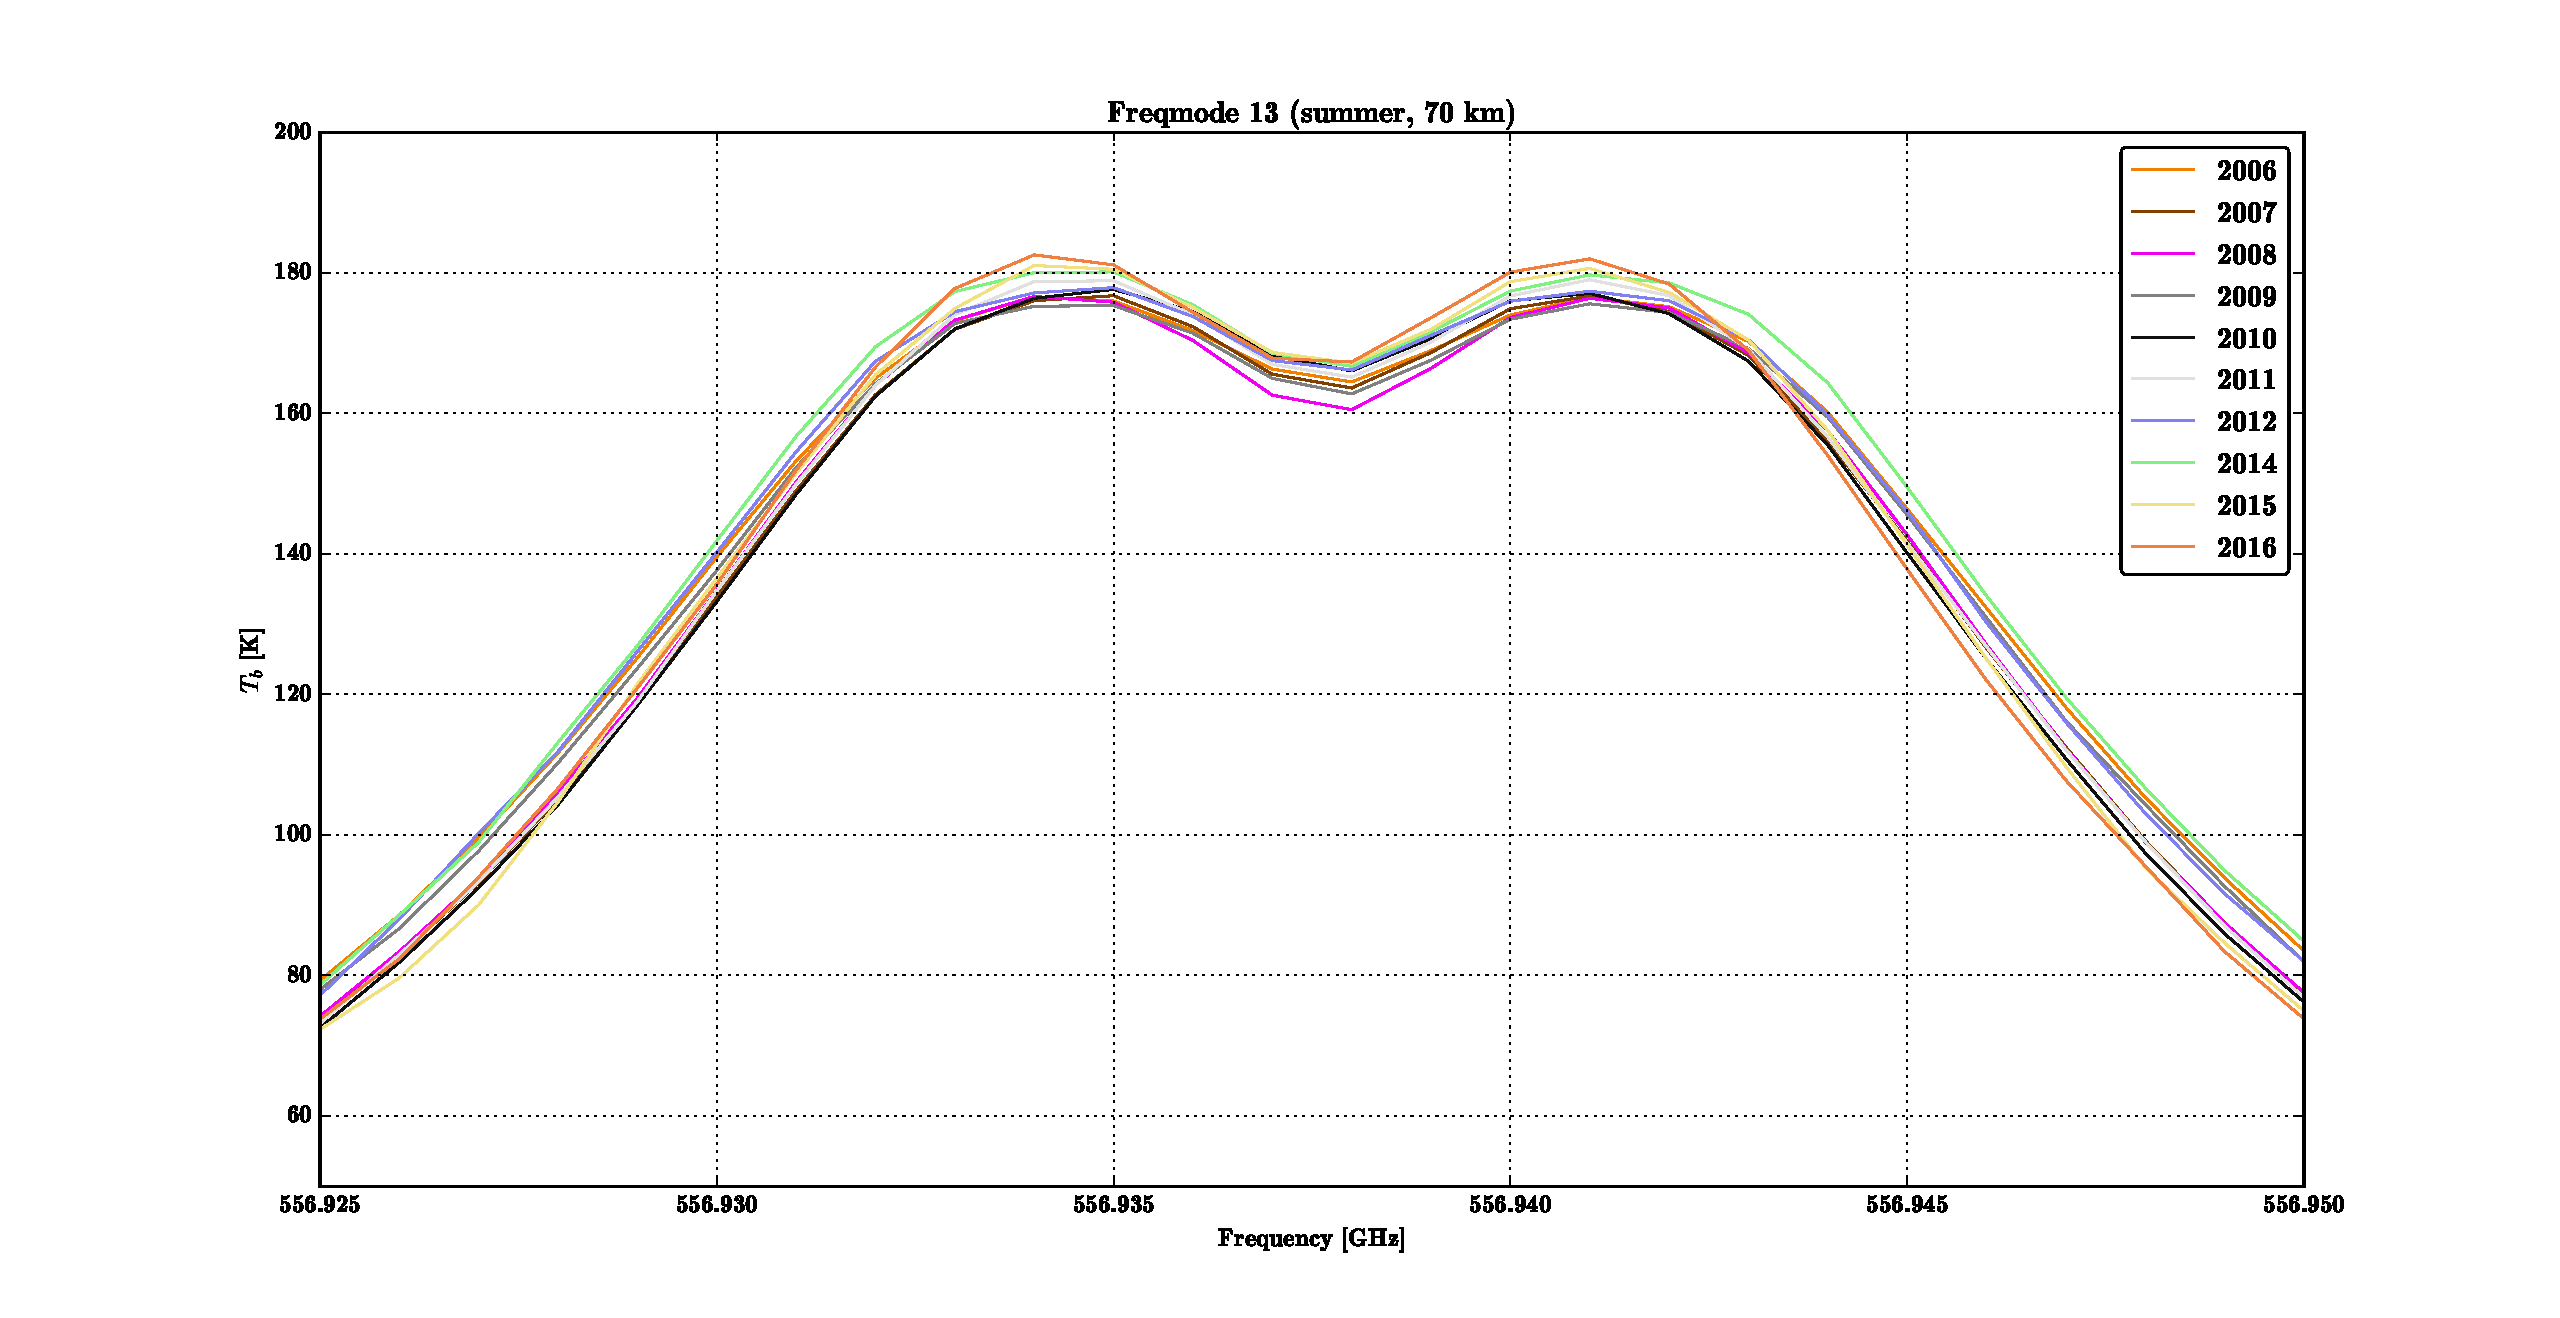
\includegraphics[width=\textwidth]{fm_13_spectra_summer_zoom.pdf}
        \caption{winter}\label{fig:spectra:13:winter:closeup}
    \end{subfigure}
    \caption{Close-up of \chem{H_2O} peak in annual median spectra for
        frequency~mode~13 for altitude interval
        65--75~km}\label{fig:spectra:13:closeup}
\end{figure}

\subsection{Sideband leakage}
\label{FM13:sbl}
There are unfortunately no sideband peaks distinct enough in the received
spectra for any conclusions to be drawn regarding the sideband leakage for
this frequency mode.

\subsection{Seasonality}
\TODO{FM13 seasonality}
